\documentclass{standalone}
\usepackage{tikz}

\definecolor{CoolBlue}{HTML}{135984}
\definecolor{CoolGreen}{HTML}{8aa21a}
\definecolor{Lavender}{HTML}{b39def}

\begin{document}
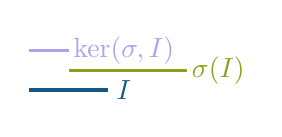
\begin{tikzpicture}
  \draw [CoolBlue, very thick] (0,0) -- (1,0) node at
  (1.2,0) {$I$};
  \draw [CoolGreen, very thick] (0.5,0.25) -- (2,0.25)
  node at (2.4,0.25) {$\sigma(I)$};
  \draw [Lavender, very thick] (0,0.5) -- (0.5,0.5) node
  at (1.2,0.5) {$\ker(\sigma, I)$};
\end{tikzpicture}
\end{document}
